% Archivo generado automáticamente con los problemas
\section*{Problems}
Sección: 23_The_renormalization_group
Páginas: 469-470
Contenido:
23.1 Consider the operator O = ¯ψ/∂ψ ¯ψ/∂ψ in QED.
(a) Evaluate the anomalous dimension of Oμν at 1-loop.
(b) If the coefficient for this operator is C = 1 at 1 TeV, what is C at 1 GeV?

23.2 Show that A = 0 in Eq. (23.38) by evaluating the anomalous dimension of GF from
Eq. (23.40) in QED. At an intermediate stage, you may want to use the Fierz identity:
 ¯ψ1PLγμγαγβψ2
 ¯ψ3PLγμγαγβψ4

= 16
 ¯ψ1PLγμψ2
 ¯ψ3PLγμψ4

,
(23.131)
which you derived in Problem 11.8.

23.3 Show that Eq. (23.97) follows from the small λR limit of the general solution to
mR(μ).

23.4 Consider a theory with N real scalar fields φi with Lagrangian
L = −1
2φi(□+ m2)φi −λ
4 (φi)2(φj)2.
(23.132)
This effective Lagrangian can describe systems with multiple degrees of freedom
near critical points (for example, the superfluid transition in 4He corresponds to
N = 2).
(a) Calculate γm and β(λR) in this theory. Check that for N = 1 you reproduce
Eqs. (23.96) and (23.95). (Note that the normalizations of λ in Eqs. (23.85)
and (23.132) are different.)
(b) Where is the location of the Wilson–Fisher fixed point in this theory in 4 −ε
dimensions?
(c) What is the value of the critical exponent ν is this theory in d = 3 in the epsilon
expansion?
Problems
451

23.5 Compute the value of the critical exponent ν in the Wilson–Fisher theory (with N =
1, as in Section 23.5.2) to order ε2.

23.6 Scheme dependence in the Wilson–Fisher theory.
(a) Compute the 1-loop RGEs in scalar φ4 theory (with Lagrangian Eq. (23.85))
using a hard cutoff. Show that you get non-zero values for λ and m at the fixed
point, but the critical exponent ν is the same as computed in Section 23.5.2.
(b) Plot the RG flow trajectories using the RGEs you just computed with a fixed
cutoff. What is different about these trajectories from those in Figure 23.1?
(c) Compute the 1-loop RGEs in the Wilsonian picture by literally integrating over
a shell in momentum from bΛ to Λ. Show that you get the same value for ν.
(d) Show that the critical exponent ν is independent of regulator and subtraction
scheme at 1-loop. Can you choose a scheme so that λ⋆and m⋆are whatever you
want?

23.7 Derive
Λ d
dΛLint(φ) =

d4p (2π)4
p2 + m2
p2
Λ2 e
p2
Λ2
δLint
δφ(p)
δLint
δφ(−p) −
δ2Lint
δφ(p)δφ(−p)
(23.133)
using the Wilson–Polchinski RGE. Show that the first term corresponds to integrat-
ing out the tree-level diagram and the second from loops.

23.8 Consider a theory with a dimension-2 mass parameter m2 and a dimensionless
coupling g.
(a) Write down and solve generic Wilsonian RGEs for this theory, as in Eqs.
(23.118) and (23.119).
(b) Fix g(ΛL) = 0.1 for concreteness with ΛL = 105 GeV. What value of m2(ΛH)
would lead to m2(ΛL) = 100 GeV?
(c) What would m2(ΛL) be if you changed m2(ΛH) by 1 part in 1020?
(d) Sketch the RG flows for this theory.

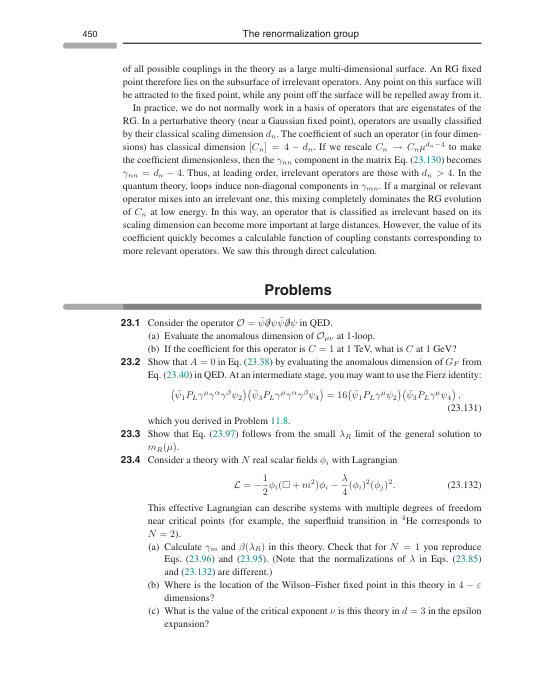
\includegraphics{./figs/23_The_renormalization_group_page_470.png}

---

